\documentclass[]{beamer}
%\documentclass[handout]{beamer}
%\usepackage[dvips]{color}
\usepackage{graphicx}
\usepackage{amsmath,amssymb,array,comment,eucal}
\newcommand{\e}{\mathbf{e}}
\renewcommand{\P}{\mathbf{P}}
\newcommand{\F}{\mathbf{F}}
\newcommand{\R}{\textsf{R}}
\newcommand{\mat}[1] {\mathbf{#1}}
%\newcommand{\ind}{\mathrel{\mathop{\sim}\limits^{\mathit{ind}}}}
%\newcommand{\iid}{\mathrel{\mathop{\sim}\limits^{\mathit{iid}}}}
\newcommand{\E}{\textsf{E}}
\newcommand{\SE}{\textsf{SE}}
\newcommand{\SSE}{\textsf{SSE}}
\newcommand{\RSS}{\textsf{RSS}}
\newcommand{\FSS}{\textsf{FSS}}
\renewcommand{\SS}{\textsf{SS}}
\newcommand{\MSE}{\textsf{MSE}}
\newcommand{\SSR}{\textsf{SSR}}
\newcommand{\Be}{\textsf{Beta}}
\newcommand{\St}{\textsf{St}}
%\newcommand{\C}{\textsf{C}}
\newcommand{\GDP}{\textsf{GDP}}
\newcommand{\NcSt}{\textsf{NcSt}}
\newcommand{\Bin}{\textsf{Bin}}
\newcommand{\NB}{\textsf{NegBin}}
\renewcommand{\NG}{\textsf{NG}}
\newcommand{\N}{\textsf{N}}
\newcommand{\Ber}{\textsf{Ber}}
\newcommand{\Poi}{\text{Poi}}
\newcommand{\Gam}{\textsf{Gamma}}
\newcommand{\BB}{\textsf{BB}}
\newcommand{\Gm}{\textsf{G}}
\newcommand{\Un}{\textsf{Unif}}
\newcommand{\Ex}{\textsf{Exp}}
\newcommand{\DE}{\textsf{DE}}
\newcommand{\tr}{\textsf{tr}}
\newcommand{\cF}{{\cal{F}}}
\newcommand{\cL}{{\cal{L}}}
\newcommand{\cI}{{\cal{I}}}
\newcommand{\cB}{{\cal{B}}}
\newcommand{\cP}{{\cal{P}}}
\newcommand{\bbR}{\mathbb{R}}
\newcommand{\bbN}{\mathbb{N}}
\newcommand{\pperp}{\mathrel{{\rlap{$\,\perp$}\perp\,\,}}}
\newcommand{\OFP}{(\Omega,\cF, \P)}
\newcommand{\eps}{\boldsymbol{\epsilon}}
\newcommand{\1}{\mathbf{1}_n}
\newcommand{\gap}{\vspace{8mm}}
\newcommand{\ind}{\mathrel{\mathop{\sim}\limits^{\rm ind}}}
\newcommand{\simiid}{\ensuremath{\mathrel{\mathop{\sim}\limits^{\rm
iid}}}}
\newcommand{\eqindis}{\ensuremath{\mathrel{\mathop{=}\limits^{\rm D}}}}
\newcommand{\iid}{\textit{i.i.d.}}
\newcommand{\SSZ}{S_{zz}}
\newcommand{\SZW}{S_{zw}}
\newcommand{\Var}{\textsf{Var}}
\newcommand{\corr}{\textsf{corr}}
\newcommand{\diag}{\textsf{diag}}
\newcommand{\var}{\textsf{var}}
\newcommand{\Cov}{\textsf{Cov}}
\newcommand{\Sam}{{\cal S}}
\def\H{\mathbf{H}}
\newcommand{\I}{\mathbf{I}}
\newcommand{\Y}{\mathbf{Y}}
\newcommand{\tY}{\tilde{\mathbf{Y}}}
\newcommand{\Yhat}{\hat{\mathbf{Y}}}
\newcommand{\Yobs}{\mathbf{Y}_{{\cal S}}}
\newcommand{\barYobs}{\bar{Y}_{{\cal S}}}
\newcommand{\barYmiss}{\bar{Y}_{{\cal S}^c}}
\def\bv{\mathbf{b}}
\def\X{\mathbf{X}}
\def\tX{\tilde{\mathbf{X}}}
\def\x{\mathbf{x}}
\def\xbar{\bar{\mathbf{x}}}
\def\Xbar{\bar{\mathbf{X}}}
\def\Xg{\mathbf{X}_{\boldsymbol{\gamma}}}
\def\Ybar{\bar{\Y}}
\def\ybar{\bar{y}}
\def\y{\mathbf{y}}
\def\Yf{\mathbf{Y_f}}
\def\W{\mathbf{W}}
\def\L{\mathbf{L}}
\def\w{\mathbf{w}}
\def\U{\mathbf{U}}
\def\V{\mathbf{V}}
\def\Q{\mathbf{Q}}
\def\Z{\mathbf{Z}}
\def\z{\mathbf{z}}
\def\v{\mathbf{v}}
\def\u{\mathbf{u}}

\def\zero{\mathbf{0}}
\def\one{\mathbf{1}}
\newcommand{\taub}{\boldsymbol{\tau}}
\newcommand{\betav}{\boldsymbol{\beta}}
\newcommand{\alphav}{\boldsymbol{\alpha}}
\newcommand{\A}{\mathbf{A}}
\def\a{\mathbf{a}}
\def\K{\mathbf{K}}
\newcommand{\B}{\mathbf{B}}
\def\b{\boldsymbol{\beta}}
\def\bhat{\hat{\boldsymbol{\beta}}}
\def\btilde{\tilde{\boldsymbol{\beta}}}
\def\tb{\tilde{\boldsymbol{\beta}}}
\def\bg{\boldsymbol{\beta_\gamma}}
\def\bgnot{\boldsymbol{\beta_{(-\gamma)}}}
\def\mub{\boldsymbol{\mu}}
\def\tmub{\tilde{\boldsymbol{\mu}}}
\def\muhat{\hat{\boldsymbol{\mu}}}
\def\t{\boldsymbol{\theta}}
\def\tk{\boldsymbol{\theta}_k}
\def\tj{\boldsymbol{\theta}_j}
\def\Mk{\boldsymbol{{\cal M}}_k}
\def\M{\boldsymbol{{\cal M}}}
\def\Mj{\boldsymbol{{\cal M}}_j}
\def\Mi{\boldsymbol{{\cal M}}_i}
\def\Mg{{\boldsymbol{{\cal M}_\gamma}}}
\def\Mnull{\boldsymbol{{\cal M}}_{N}}
\def\gMPM{\boldsymbol{\gamma}_{\text{MPM}}}
\def\gHPM{\boldsymbol{\gamma}_{\text{HPM}}}
\def\Mfull{\boldsymbol{{\cal M}}_{F}}
\def\tg{\boldsymbol{\theta}_{\boldsymbol{\gamma}}}
\def\g{\boldsymbol{\gamma}}
\def\eg{\boldsymbol{\eta}_{\boldsymbol{\gamma}}}
\def\G{\mathbf{G}}
\def\cM{\cal M}
\def\D{\Delta}
\def \shat{{\hat{\sigma}}^2}
\def\uv{\mathbf{u}}
\def\l {\lambda}
\def\d{\delta}
\def\Sigmab{\boldsymbol{\Sigma}}
\def\Lambdab{\boldsymbol{\Lambda}}
\def\lambdab{\boldsymbol{\lambda}}
\def\Mg{{\cal M}_\gamma}
\def\S{{\cal{S}}}
\def\qg{p_{\boldsymbol{\gamma}}}
\def\pg{p_{\boldsymbol{\gamma}}}
\def\t{\boldsymbol{\theta}}  
\def\T{\boldsymbol{\Theta}}  
\usepackage{verbatim}

\usetheme{Warsaw}
\title{Checking Assumptions: Residuals  and Influential Observations}
\subtitle{Merlise Clyde}
\author{STA721 Linear Models}
\institute{Duke University}
\date{\today}
\logo{duke.eps}

\begin{document}
\maketitle

\begin{frame}\frametitle{Outline}
Topics
  \begin{itemize}
  \item Distribution of Residuals
  \item Leverage
  \item Standardized Residuals
  \item Cook's Distance
  \item Example: Stackloss data

  \end{itemize}


Readings: Christensen  Chapter 13
\end{frame}
%\section{Models}
\begin{frame} \frametitle{ Linear Model}
Linear Model:
 $$ \Y = \mub + \eps $$ \pause
Assumptions: \pause
\begin{eqnarray*}
   \mub \in C(\X) & \Leftrightarrow & \mub = \X \b \pause \\
  \eps  & \sim &  \N(\zero_n, \sigma^2 \I_n) \pause
\end{eqnarray*}
What could go wrong?
\begin{itemize}
  \item  Wrong mean \pause \\
\item Wrong covariance  \pause \\
\item Wrong distribution for $\eps$  \\
\end{itemize}
\end{frame}
\begin{frame}
  \frametitle{Residuals}
  Residuals  (MLE of $\eps$) are
  \begin{eqnarray*}
\e & =  & \Y - \X \bhat    \pause \\
  & = & (\I_n - \P_\X) \Y  \pause \\
 &   & \\
\E[\e] & = &  (\I_n - \P_\X)\mub  \pause \\
       & = & \zero_n \text{ if } \mub \in C(\X)  \pause
  \end{eqnarray*}
Mean will not be zero if we have left out terms
\end{frame}

\begin{frame}
  \frametitle{Variance Residuals}
  Under model with constant variances $\Cov[\Y] = \sigma^2 \I_n$ \pause
  \begin{eqnarray*}
\Cov=[\e] & = & \Cov[(\I - \P_\X) \Y  \pause \\
 & = & (\I- \P_\X)^T \Cov[\Y](\I - \P_\X)    \pause \\
& = & \sigma^2(\I- \P_\X)^T(\I - \P_\X)  \pause \\ 
& = & \sigma^2 (\I - \P_\X)   \pause \\
& & \\
\e & \sim & \N( \zero,  \sigma^2 (\I - \P_\X) )  \pause
  \end{eqnarray*}
  \begin{itemize}
  \item $\P_\X$ is the ``hat'' matrix (sometimes called $\H =
    [h_{ij}]$)  \pause
  \item diagonal elements of $\P_\X$ are denoted as $h_{ii}$  \pause
  \item leverage of the $i$th observation is $h_{ii}$ \pause
  \end{itemize}
$$\var(e_i) = \sigma^2(1 - h_{i})$$
\end{frame}

\begin{frame}
  \frametitle{Parameterization}
  Let $\X = [\one_n \Z ]$ and $\P_\one = \one( \one^T \one)^{-1}
  \one^T$ denote the projection on $C(\one)$  \pause
  \begin{eqnarray*}
\Y  & = & \X \b + \eps  \pause \\
 & = & \one_n \alpha_0 + \Z \alphav + \eps   \pause \\
    & = & \one_n \alpha_0 + \P_\one\Z \alphav + (\I_n - \P_\one)\Z
    \alphav + \eps  \pause
    \\
& & \\ & & \\ & & \\
& & \\ & & \\ & & \\
    & = &  \one_n \alpha_0^* + (\Z - \one_n \bar{\Z}^T) \alphav + \eps 
  \end{eqnarray*}

\end{frame}
\begin{frame}
  \frametitle{Mahalanobis Distance \& Leverage}
Let $z_i^T$ denote the vector of explanatory variables for the $i$th case   \pause
  \begin{eqnarray*}
\P_\X&  = &  \P_\one + \P_{\Z - \one \bar{\Z}^T}  \pause \\    
    &  &  \\
h_{ii} & = & \frac{1}{n} + (z_i - \bar{\Z})^T 
\left( 
(\Z - \one \bar{\Z}^T)^T(\Z - \one \bar{\Z}^T)
\right)^{-1} 
(z_i - \bar{\Z})  \pause \\
 & = & \frac{1}{n} + \frac{D^2_i}{n-1}  \pause
  \end{eqnarray*}
Leverage is a function of  the estimated Mahalanobis distance $D_i^2$ of $z_i$ from $\bar{\Z}$
\end{frame}

\begin{frame}
  \frametitle{Residual Plots}
  Under normality and constant variance assumptions,  the residuals
  $\e$ and fitted values $\Yhat$ are jointly normal but independent.
 \pause
Under the correct model
 \pause
  \begin{itemize}
    \item  $\E[\e] = \zero_n$:  scatter plots of residuals versus any
      combination of  terms in the mean function will have a constant
      mean of $\zero$  \pause
    \item $\var(e_i) = \sigma^2(1 - h_{ii})$, so even if fitted model
      is correct, the variances are not constant.  Lower variability
      for points with high leverage with $h_{ii} \approx 1$ \pause
  \item The residuals are correlated, but this correlation is usually
    not visible in residual plots  \pause 
    
  \end{itemize}
When the model is not correct we hope to see structure in the residual
plots to help us re-model the data  \pause

Use standardized residuals


\end{frame}
\begin{frame}
  \frametitle{Standardized Residuals}
Since $\var(e_i) = \sigma^2( 1 - h_{ii})$ has non-constant variance
 \pause
\begin{itemize}
\item 
Divide by standard deviation:  $$\frac{e_i}{\sigma \sqrt{1 -
    h_{ii}}}$$ (constant variance)  \pause

\item (Internally) Standardized residuals $$r_i =  \frac{e_i}{\hat{\sigma} \sqrt{1 -
    h_{ii}}}$$
where $\hat{\sigma}$ is root MSE  \pause
\end{itemize}

\end{frame}

\begin{frame}
  \frametitle{Properties of Leverage}
  \begin{itemize}
  \item $\sum_i h_{ij} = 1$  \pause
    \begin{eqnarray*}
 \one^T\P_\X &  = &  \one^T \P_\one + \one^T \P_{\Z - \one \bar{\Z}^T}
  \pause \\
 & = & \one^T \one (\one^T\one)^{-1} \one^T + \zero^T   \pause \\
 & = &    \one^T  \pause
    \end{eqnarray*}

  \item  $ 0 \leq h_{ii} \leq 1$  \pause
    \begin{eqnarray*}
     \P_\X &  = &\P_\X^2  \pause\\
    h_{ii} & = & \sum_j h_{ij} h_{ji} \pause \\
          & = & \sum_j h_{jj}^2  \pause \\
          & = & h_{ii}^2 +  \sum_{j \neq i} h_{jj}^2   \pause \\
h_{ii}(1 - h_{ii}) & \geq 0
    \end{eqnarray*}
  \end{itemize}
  \end{frame}

  \begin{frame}
    \frametitle{Predictions}
$$\hat{Y}_i =  h_{ii} Y_i  + \sum_{j \neq i} h_{ij} Y_j$$  \pause


If $h_{ii} \approx 1$ then $  \hat{Y}_i   \approx Y_i$   \pause
  
    \begin{itemize}
\item $\sum_j h_{ij} = 1$  \pause
\item $\sum_i h_{ij}^2 = 1$  \pause
    \begin{eqnarray*}
 \one^T\P_\X &  = &   \one^T (\P_\one + \P_\X)(\P_\one + \P_\X)^T
 \pause  \\
 & = & \one^T \one (\one^T\one)^{-1} \one^T + \zero^T   \pause \\
 & = &    \one^T  \pause
\end{eqnarray*}
\item $h_{ij} \approx 0$ for $i \neq j$ if $h_{ii} \approx 1$  \pause

\item $\var(e_i) = \sigma^2 (1 - h_{ii}) \approx 0$ if $h_{ii} \approx 1$ 
   
    \end{itemize}
  \end{frame}
  \begin{frame}
    \frametitle{Illustration}
    
  \end{frame}

  \begin{frame}
    \frametitle{Predicted Residuals}
    Let $\X_{(i)}$ and $\Y_{(i)}$ denote the design matrix and
    response vector with the $i$th row $\x_i^T$ deleted  \pause
    \begin{itemize}
\item       $\bhat_{(i)} = (\X_{(i)}^T\X_{(i)})^{-1 }\X_{(i)}^T
  \Y_{(i)}$  \pause
\item Predicted residual $\e_{(i)}  = y_i - \x_{(i)}^T \bhat_{(i)}$  \pause
\item Variance $\var(e_{(i)}) = \sigma^2( 1 +
  \x_{(i)}^T(\X_{(i)}^T\X_{(i)})^{-1} \x_{(i)})$  \pause
    \end{itemize}

  \end{frame}
  \begin{frame}
    \frametitle{Updating Formula}
    How to compute without re-fitting model for each case deletion?  \pause
$$ \X_{(i)}^T \X_{(i)} = \X^T\X + \frac{(\X^T\X)^{-1} \x_i \x_i^t
  (\X^T\X)^{-1}}
{1 - \x_i^T (\X^\X)^{-1} \x_i}$$  \pause
Special case of the Binomial Inverse Theorem or Woodbury Theorem  \pause

\begin{eqnarray*}
  \bhat_{(i)} & = & (\X_{(i)}^T\X_{(i)})^{-1 }\X_{(i)}^T
  \Y_{(i)}  \pause \\
 & = & (\X_{(i)}^T\X_{(i)})^{-1 }(\X^T\Y - \x_i y_i)  \pause \\
 &  & \text{ some algebra}  \pause \\
 & = & \bhat + \frac{ \X^T\X \x_i e_i}{ 1 - h_{ii}}   \pause
\end{eqnarray*}

≈

  \end{frame}
  \begin{frame}
    \frametitle{Predicted Residuals}
    Predicted residual
$$ e_{(i)} = y_i - \x_i^T \bhat{(i)} = \frac{e_i}{1 - h_{ii}}$$
 \pause
with variance
$$\var(e_{(i)}) = \frac{\sigma^2}{1 - h_{ii}}$$
 \pause
Standardized predicted residual is 
$$\frac{e_{(i)}}{\sqrt{\var(e_{(i)})}}  = \frac{e_i/(1 -
  h_{ii})}{\sigma/\sqrt{1 - h_{ii}}} = \frac{e_i}{\sigma \sqrt{1 -
    h_{ii}} }
$$ \pause
Same as before!
  \end{frame}
  \begin{frame}
    \frametitle{External estimate of $\sigma^2$}
    Estimate $\shat_{(i)}$ using data with case $i$ deleted  \pause
    \begin{eqnarray*}
\SSE_{(i)} & = &  \SSE - \frac{e_i^2}{1 - h{ii}}  \pause \\
\shat_{(i)} = \MSE_{(i)} & = &  \frac{\SSE_{(i)}}{n - p - 1}  \pause\\
    \end{eqnarray*}
Externally Standardized residuals  \pause
$$t_i = \frac{e_{(i)}}{\sqrt{\shat_{(i)}/(1 - h_{ii})}}  =  \frac{y_i
  - \x_i^T \bhat_{(i)}} {\sqrt{\shat_{(i)}/(1 - h_{ii})}}$$  \pause

May still miss extreme points with high leverage, but will pick up unusual $y_i$s
  \end{frame}
  \begin{frame}
    \frametitle{Outlier Test}
    H$_0$: $\mu_i = \x_i^T \b$  versus H$_a$: $\mu_i = \x_i^T\b +
    \alpha_i$  \pause
    \begin{itemize}
    \item  Show that t-test for testing H$_0$: $\alpha_i = 0$ is equal
      to $t_i$ (HW)  \pause
  \item if p-value is
small declare the $i$th case to be an outlier:  $\E[Y_i]$ not given by
$\X \b$  but $\X\b = \delta_i \alpha_i$    \pause
\item control for multiple testing  \pause
\item Extreme case $\mub = \X\b + \I_n \alphav$  all points have their
  own mean!   \pause
    \end{itemize}
  \end{frame}
  \begin{frame}
    \frametitle{Cook's Distance}
    Cook's Distance  measure of how much predictions change with $i$th
    case deleted  \pause
    \begin{eqnarray*}
D_i & =  &\frac{\| \Y_{(i)} - \Y \|^2}{ p \shat} = 
\frac{ (\bhat_{(i)} - \bhat)^T \X^T\X (\bhat_{(i)} - \bhat) }{ p
  \shat}  \pause \\
& = & \frac{r_i^2}{p} \frac{h_{ii}}{ 1 - h_{ii}}  \pause
    \end{eqnarray*}
Flag cases where $D_i > 1$ or large relative to other cases
 \pause
\vspace{18pt}
Influential Cases
  \end{frame}
  \begin{frame}
   \frametitle{Stackloss Data}
\vspace{-24pt}
    \centerline{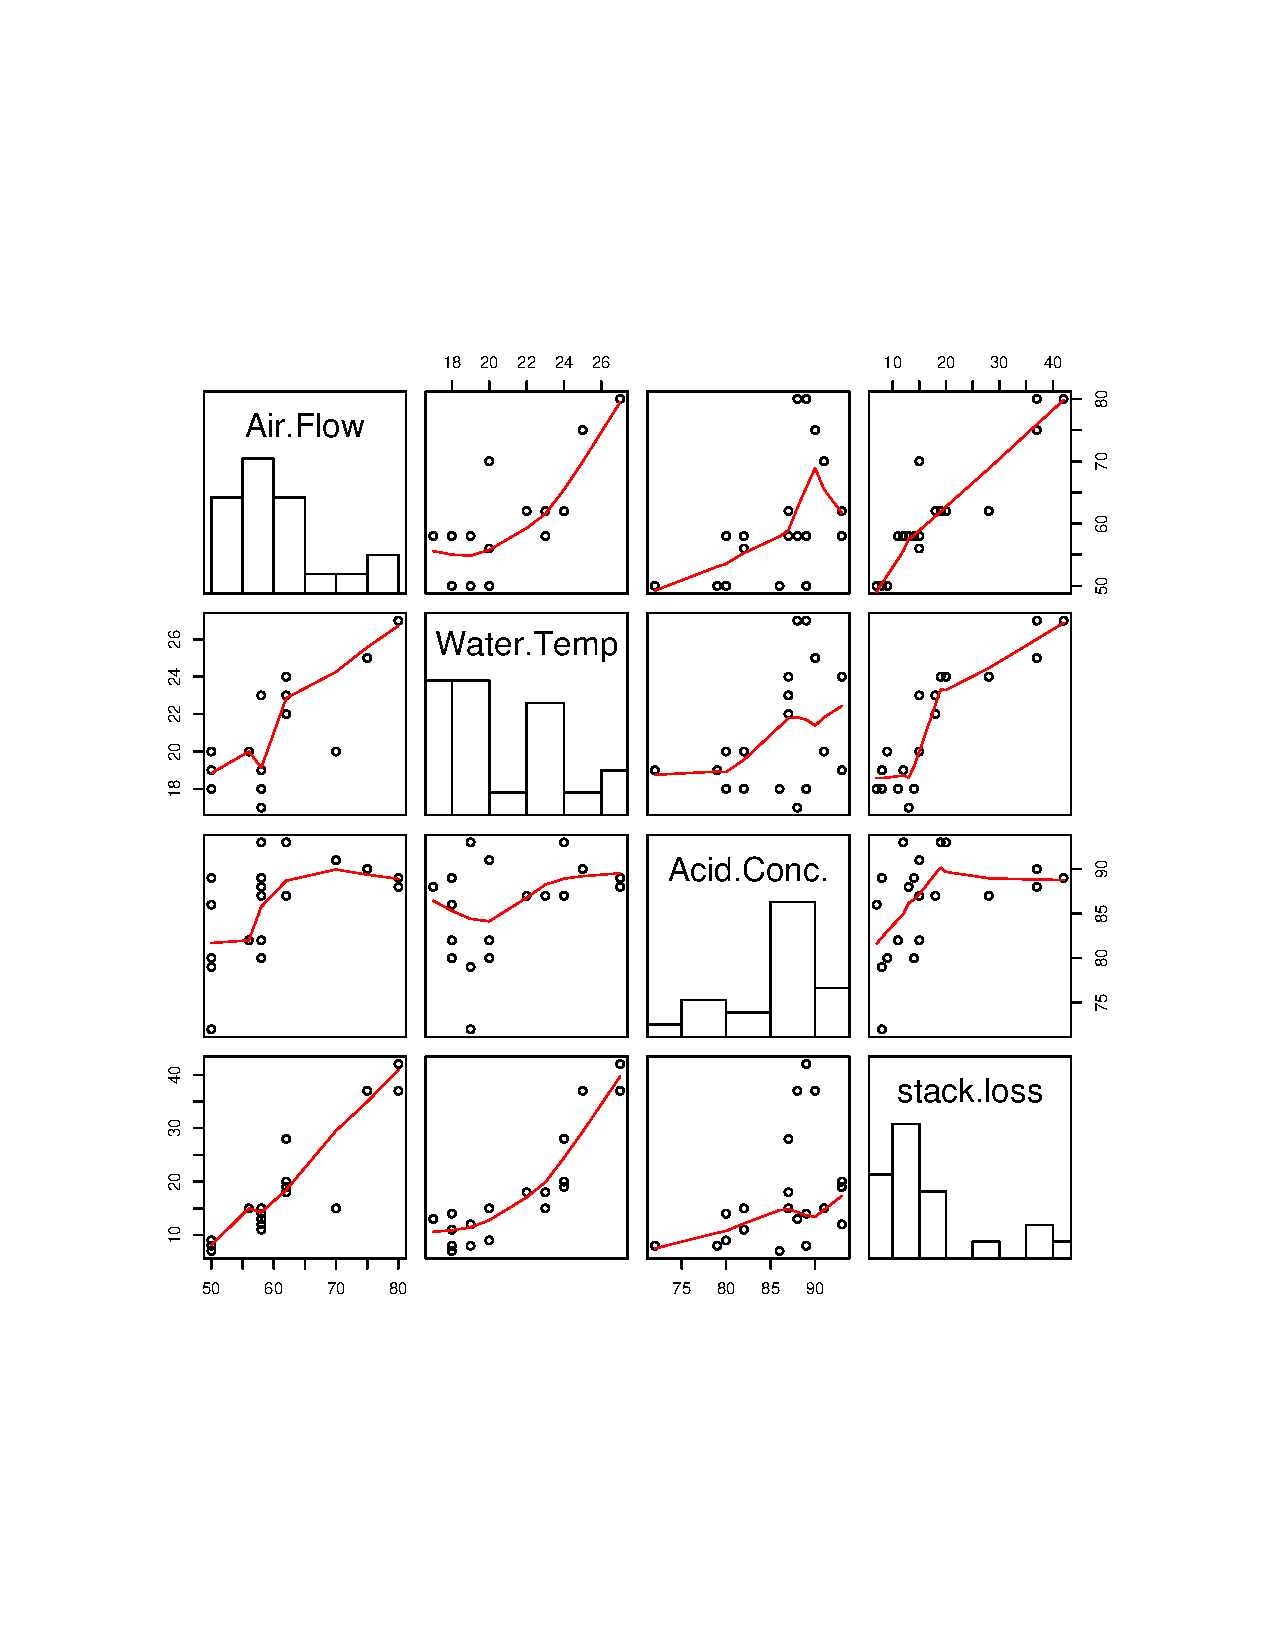
\includegraphics[height=4in]{stackloss-pair}}
  \end{frame}
  \begin{frame}
    \frametitle{Stackloss Added Variable Plot}
    \centerline{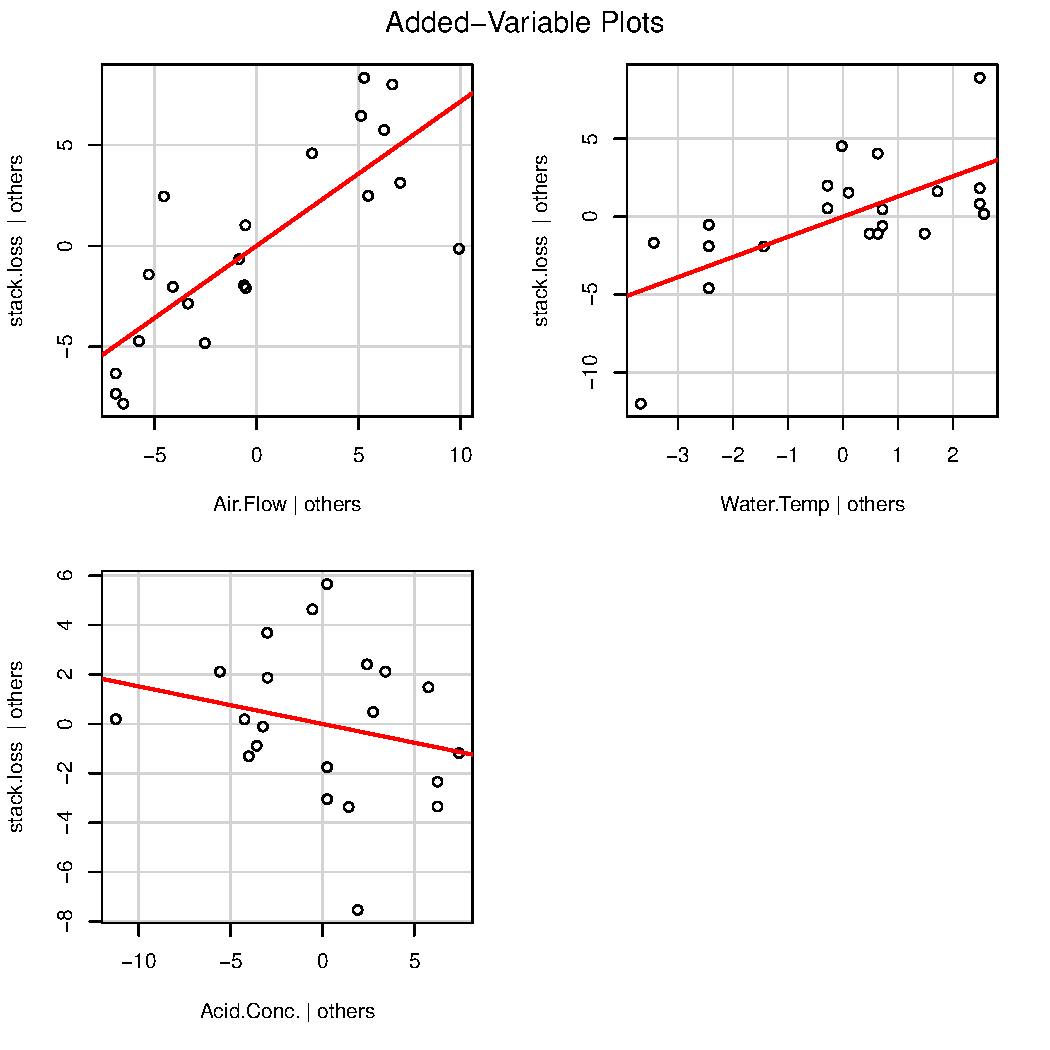
\includegraphics[height=3.5in]{stackloss-avp}}
  \end{frame}
  \begin{frame}
    \frametitle{Stackloss Data}
    \centerline{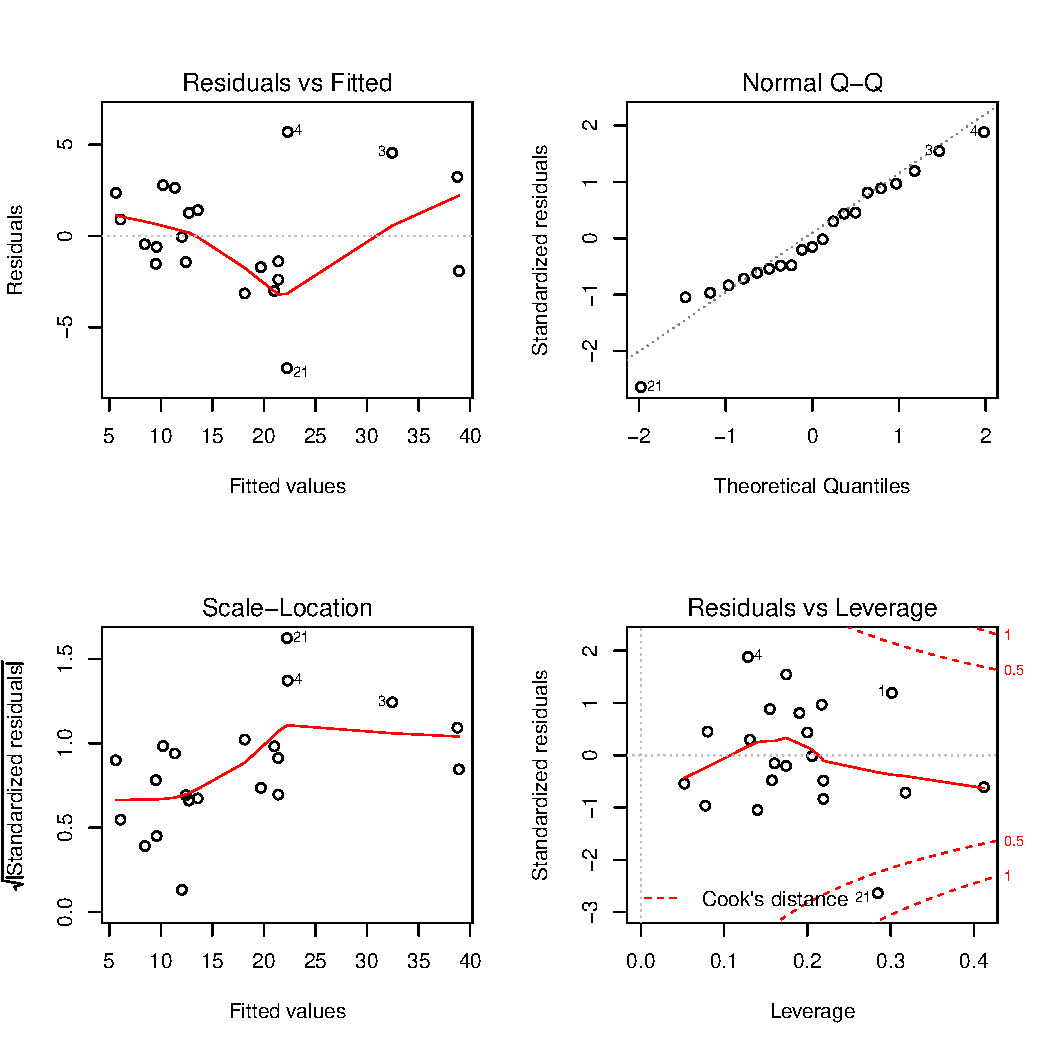
\includegraphics[height=3.5in]{stackloss-resid}}
  \end{frame}
  \begin{frame}
    \frametitle{Case 21}
    \begin{itemize}
    \item Leverage $0.285$
\item Cooks'd Distance $.69$
\item p-value $t_{21}$ is $0.0042$
\item Bonferonni adjusted p-value is $0.0024$
\item Other points?  Masking?  
\item Refit without Case 21
    \end{itemize}
Others have suggested that cases (1, 3, 4, 21) are outliers
  \end{frame}
  \begin{frame} \frametitle{To Remove or Not?}
    \begin{itemize}
    \item  For suspicious cases, check data sources  \pause
    \item  Check that points are not outliers because of wrong mean
      function or distributional assumptions  \pause
   \item Influential cases - report results with and without cases
     (resutls may change)  \pause
   \item Outlier test - suggests alternative population; if not
     influential may in keep analysis, but will inflate $\shat$ and
     interval estimates   \pause
   \item Document steps - reproducibility!
   \item Robust Regression Methods  \pause
    \end{itemize}
Are there outliers in the Stackloss Data?
  \end{frame}
\end{document}


